\chapter{Estudo Experimental}
\label{cap:avaliacao}

Neste capítulo será apresentado o processo de avaliação utilizado para verificar a precisão do sistema de detecção de quedas proposto. Espera-se que o SafeWatch apresente uma precisão similar aos demais sistemas de detecção de quedas presentes na literatura.

As seções desse capítulo são organizadas da seguinte maneira: A Seção \ref{sec:metodology} apresenta os detalhes da metodologia utilizada para avaliar o SafeWatch; A Seção \ref{sec:metrics} mostra as métricas utilizadas na avaliação; A Seção \ref{sec:results} apresenta os resultados obtidos no experimento realizado e faz uma comparação com os resultados obtidos em outros trabalhos.



\section{Metodologia}
\label{sec:metodology}

Para avaliarmos o desempenho do SafeWatch foi realizado uma série de experimentos. O algoritmo de detecção de quedas proposto foi avaliado através de um conjunto de quedas simuladas e também um conjunto de atividades diárias realizadas pelos participantes do experimento. O grupo de voluntários possui um perfil diversificado, sendo composto de 3 homens e 5 mulheres como pode ser visto na Tabela \ref{tab:experiment}. O experimento não foi realizado com nenhum idoso devido a grande dificuldade de simular eventos de queda sem por em risco a integridade física do mesmo. Além disso, as base de dados encontradas referentes a eventos de quedas com idosos são privadas e não foram disponibilizadas, como vista no trabalho proposto por \cite{kostopoulos2015f2d}.


\begin{table}
	\centering
	\caption{Participantes do experimento}
	\label{tab:experiment}
	\begin{tabular}{c|c|c|c|c}
		\hline
		\textbf{Indivíduo}  & \textbf{Idade} 	& \textbf{Sexo}   &    \textbf{Peso}    & \textbf{Altura} 	 \\
		Indivíduo 1         &    28          & Masculino            & 82kg      		& 1.80m          \\  
		Indivíduo 2         &    20          & Feminino             & 63kg      		& 1.63m          \\
		Indivíduo 3         &    25          & Feminino             & 62kg      		& 1.59m          \\ 
		Indivíduo 4         &    29          & Masculino            & 130kg      		& 1.65m          \\ 
		Indivíduo 5         &    27          & Feminino             & 57kg      		& 1.69m          \\ 
		Indivíduo 6         &    14          & Feminino             & 45kg      		& 1.62m          \\
		Indivíduo 7         &    20          & Masculino            & 88kg      		& 1.80m          \\ 
		Indivíduo 8         &    30          & Feminino             & 62kg      		& 1.55m          \\   
	\end{tabular}
\end{table}

 
O smartwatch escolhido para realizar o experimento foi um \textit{Moto 360} da 1º geração com as seguintes características \citep{moto360}:

	\begin{enumerate}
		\item Sistema Operacional: Android Wear 2.0.
		\item CPU: Qualcomm Snapdragon 400, 1.2 GHz.
		\item Memória RAM: 512 MB.
		\item Capacidade de Armazenamento: 4 GB.
	\end{enumerate}
	
Já o smartphone escolhido foi um \textit{LG G2} com as seguintes características \citep{lg_g2}:

	\begin{enumerate}
		\item Sistema Operacional: Android  Lollipop 5.0.2.
		\item CPU: Quad-core 2.26 GHz Krait 400.
		\item Memória RAM: 2 GB.
		\item Capacidade de Armazenamento: 16GB.
	\end{enumerate}


Para avaliar o algoritmo de detecção de quedas implementado, foi realizado o seguinte experimento, composto de três etapas:

\begin{itemize}
	\item{\textbf{Preparação}: Nesta etapa é solicitado que o usuário coloque o smartwatch em seu pulso e ajuste a pulseira do relógio de uma maneira que o smartwatch permaneça firme, mas confortável. Depois disso, é informado que o usuário deverá simular duas quedas em cada um dos sentidos escolhidos: Costas, Frontal, Lado Direito, Lado Esquerdo. A ordem das quedas é decidida pelo usuário, o único requisito é que ele realize todas as oito quedas. }
	
	\item{\textbf{Realização das Quedas}: O usuário irá se posicionar de pé, na frente de um colchão coberto de almofadas como pode ser visto na Figura \ref{fig:fall_image}. A partir desta posição, ele irá realizar as oitos quedas, duas de cada tipo, como descrito na etapa anterior. A ordem das quedas é escolhida pelo usuário.  }
	
	\item{\textbf{Realização de Atividades Diárias}: Nesta etapa solicitamos que o usuário realize 4 atividades do seu cotidiano. Elas são: sentar em uma cadeira, levantar de uma cadeira, deitar no colchão e levantar do colchão. Estas atividades são realizadas afim de verificar se o sistema proposto é capaz de distinguir atividades diárias de um evento de queda. O sistema proposto não é capaz de distinguir qual a atividade diária que está sendo realizada, ele só é capaz de diferencia-la de um evento de queda.}
	
	
\end{itemize}


Além de executarem as simulações de queda antes das atividades diárias, ambos os eventos foram executados de maneira isolada, ou seja, não foi seguida nenhuma ordem ou sequência pré-definida de eventos. 

\begin{figure}[ht]
	\centering
	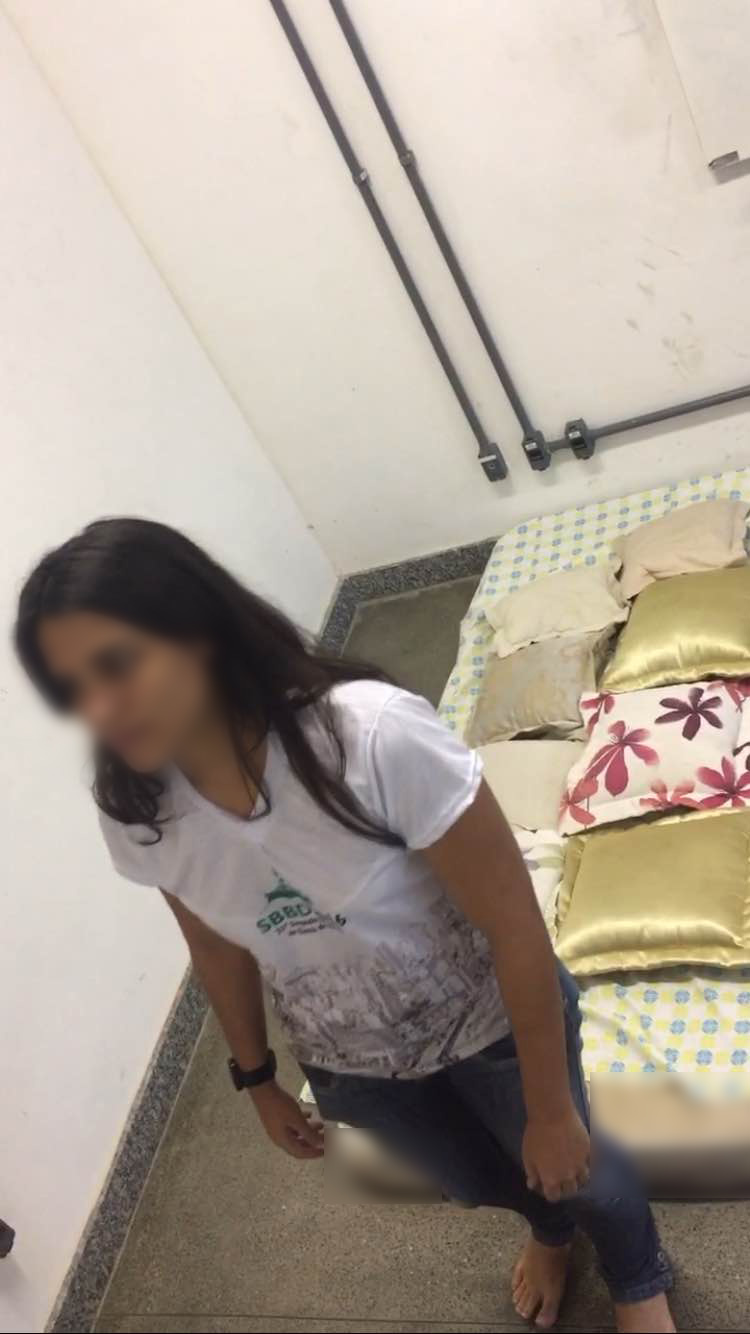
\includegraphics[scale=0.25]{imagens/fall_image.png}
	\caption{Usuário em preparação para uma queda de costas. Figura Elaborada pelo autor (2016).}
	\label{fig:fall_image}
\end{figure} 


\section{Métricas de Avaliação}
\label{sec:metrics}

Para que possamos analisar a performance do sistema de detecção de quedas foram utilizadas três métricas, a \textit{Sensibilidade},  \textit{Especificidade} e \textit{Acurácia}. De acordo com \cite{casilari2015automatic}, os valores de \textit{Sensibilidade} e \textit{Especificidade} são duas métricas bastante utilizadas na literatura para a análise de performance em sistemas de detecção de quedas. Elas representam, respectivamente, a proporção de eventos de queda e \ac{AD} que foram classificadas corretamente como tal. Já a \textit{Acurácia} é uma combinação da \textit{Sensibilidade} e da \textit{Especificidade} e nos dá uma ideia geral da performance do sistema.

A \textit{Sensibilidade} é expressa pela fórmula \ref{eq:Sensibilidade}. As variáveis \textit{TP} e \textit{FN} são, respectivamente, acrónimos para True Positive (Verdadeiro Positivo em inglês) e False Negative (Falso Negativo em inglês). A variável TP representa o número de eventos de queda corretamente classificadas, enquanto FN representa as quedas que não foram detectadas pelo sistema.

\begin{equation}
Sensibilidade = \frac{TP}{TP + FN}
\label{eq:Sensibilidade}
\end{equation}


Já a \textit{Especificidade} é expressa pela fórmula \ref{eq:Especificidade}. As variáveis \textit{TN} e \textit{FP} são, respectivamente acrónimos para True Negative (Verdadeiro Negativo em inglês) e False Positive (Falso Positivo em inglês). A variável TN representa o número de atividades diárias corretamente classificadas como tal, enquanto FP representa as atividades diárias que foram classificadas como queda.

\begin{equation}
Especificidade = \frac{TN}{FP + TN}
\label{eq:Especificidade}
\end{equation}

Para calcularmos a acurácia geral do sistema, devemos utilizar a fórmula \ref{eq:accuracy}. 

\begin{equation}
Acuracia = \frac{TP + TN}{TP + FP + TN + FN}
\label{eq:accuracy}
\end{equation}


\section{Resultados}
\label{sec:results}

Na tabela \ref{tab:results_fall} podemos ver os resultados dos experimentos de queda para cada um dos indivíduos. Como descrito na Seção \ref{sec:metodology} cada individuo realizou duas quedas em quatro sentidos diferente. Cada elemento da tabela representa o número de quedas que foram identificadas com sucesso pelo sistema em cada uma das direções. 

\begin{table}[h]
	\centering
	\caption{Resultados do experimentos de Queda.}
	\label{tab:results_fall}
	\begin{tabular}{c|c|c|c|c}
		\hline
		\textbf{Individuo}  & \textbf{Frente} 	& \textbf{Costas}   &    \textbf{Direita}    & \textbf{Esquerda} 	 \\
		Individuo 1         & 2        		    & 1            		& 2      		 		 & 2         \\  
		Individuo 2         & 1        		    & 2            		& 2      		 		 & 2         \\
		Individuo 3         & 2        		    & 2            		& 1      		 		 & 2         \\
		Individuo 4         & 2        		    & 2            		& 2      		 		 & 2         \\
		Individuo 5         & 2        		    & 1            		& 2      		 		 & 1         \\
		Individuo 6         & 2        		    & 2            		& 2      		 		 & 1         \\
		Individuo 7         & 2        		    & 2            		& 2      		 		 & 2         \\
		Individuo 8         & 2        		    & 1            		& 2      		 		 & 2         \\
	\end{tabular}
\end{table}


Como podemos ver na tabela \ref{tab:results_fall}, o número de verdadeiros-positivos é de 57, enquanto o número de falsos-negativos é de somente 7, o que nos dá uma \textit{especificidade} de $89,06\%$. Foi possível observar que o limiar inicial de $6G$ no algoritmo de detecção de quedas não foi alcançado em todos os eventos erroneamente não categorizados como queda.


Já na tabela \ref{tab:results_adl}, podemos ver os resultados do experimentos de \ac{AD} para cada um dos indivíduos. Cada um deles realizou quatro tipos de \ac{AD}, como descrito na Seção \ref{sec:metodology}. Cada elemento da tabela representa o número de \ac{AD} que não foram identificadas pelo sistema como um evento de queda. 


\begin{table}[h]
	\centering
	\caption{Resultados do experimentos de Atividades Diárias.}
	\label{tab:results_adl}
	\begin{tabular}{c|c|c|c|c}
		\hline
		\textbf{Individuo}  & \textbf{Levantar(Cadeira)} 	& \textbf{Sentar(Cadeira)}   &    \textbf{Levantar(Cama)}    & \textbf{Deitar(Cama)} 	 \\
		Individuo 1         & 2        		    & 2            		& 2      		 		 & 2         \\  
		Individuo 2         & 2        		    & 2            		& 2      		 		 & 2         \\
		Individuo 3         & 2        		    & 2            		& 2      		 		 & 2         \\
		Individuo 4         & 2        		    & 2            		& 2      		 		 & 2         \\
		Individuo 5         & 2        		    & 2            		& 2      		 		 & 2         \\
		Individuo 6         & 2        		    & 2            		& 2      		 		 & 2         \\
		Individuo 7         & 2        		    & 2            		& 2      		 		 & 2         \\
		Individuo 8         & 2        		    & 2            		& 2      		 		 & 2         \\
	\end{tabular}
\end{table}

 

Neste experimento, nenhum dos 64 eventos \ac{AD} foi identificado como um evento de queda pelo sistema, levando a uma \textit{especificidade} de $100\%$. De forma geral o sistema possui uma \textit{acurácia} de $94,53\%$.


Como visto na Tabela \ref{tab:compare}, o algoritmo proposto neste trabalho apresentou resultados satisfatórios identificando um evento de queda em quase $90\%$ dos casos, e não apresentando nenhum falso-positivo nas \ac{AD} testadas. Em comparação com o Speedy, sistema desenvolvido por \cite{degen2003speedy}, o nosso sistema apresentou uma sensibilidade $24,06\%$ maior, ou seja, o SafeWatch apresentou uma especificidade de $89,06\%$ contra $65\%$ do Speedy em experimentos bastantes similares.

\begin{table}[h]
	\centering
	\caption{Comparação com os resultados dos Trabalhos Relacionados.}
	\label{tab:compare}
	\begin{tabular}{c|c|c|c|c}
		\hline
		\textbf{}  & \textbf{SafeWatch} 	& \textbf{Speedy}   &    \textbf{F2D}    & \textbf{Sistema de Detecção de Pulso} 	 \\
		Sensibilidade         & 89,06\%        		    & 65\%           & 93,48\%      		 		 & 95\%         \\  
		Especificidade        & 100\%        		    & -           	 & 98,54\%      		 		 & 96,07\%         \\
		Acurácia        	  & 94,53\%        		    & -              & 96,01\%      		 		 & 95,85\%         \\

	\end{tabular}
\end{table}

Entretanto em comparação com \cite{hsieh2014wrist}, este trabalho apresentou uma \textit{sensibilidade} $5,94\%$ menor e uma \textit{especificidade} $3,3\%$ maior. Um dos prováveis motivos desse valor menor de \textit{Sensibilidade} são as condições do experimento.  Os experimentos realizados por \cite{hsieh2014wrist} foram em uma superfície acolchoada mais fina que um colchão convencional, o que leva a uma aceleração maior no impacto, podendo diminuir o número de falsos-negativos no experimento realizado. Em relação ao tipos de quedas realizados, tanto este, quanto o trabalho proposto por \cite{hsieh2014wrist} apresentaram quatro tipos de quedas: frontais, laterais (Direito e Esquerdo), Costas. Já em relação as \ac{AD}, ele apresentou um número maior de atividades, incluindo andar e correr, o que pode levar a número maior de falso-positivos. 






